\documentclass[journal]{IEEEtran}

\usepackage[utf8]{inputenc}
\usepackage[T1]{fontenc}
\usepackage{amsmath,amssymb,amsfonts}
\usepackage{algorithmic}
\usepackage{graphicx}
\usepackage{booktabs}
\usepackage{multirow}
\usepackage{xcolor}
\usepackage{url}
\usepackage{cite}
\usepackage{hyperref}
\hypersetup{
    colorlinks=true,
    linkcolor=blue!60!black,
    citecolor=blue!60!black,
    urlcolor=blue!60!black
}
\usepackage{tikz}
\usetikzlibrary{positioning,shapes.geometric,arrows.meta,fit,backgrounds,calc}
\usepackage[skip=2pt]{caption}
\usepackage{array}

\begin{document}

\title{NeuroKV: Adaptive Hierarchical Key--Value Cache Management via Deep Reinforcement Learning for Long-Context Large Language Model Inference\\
\large{\textit{Deep Learning -- Final Project Proposal}}}

\author{[Author Name]\\
School of [Department], Shanghai Jiao Tong University\\
\textit{Email: [author@sjtu.edu.cn]} \\
\textit{Proposal Date: May 11, 2026}
}

\maketitle

\begin{abstract}
Long-context large language models (LLMs) have become foundational to retrieval-augmented generation, agent workflows, and multi-document reasoning, but their deployment is bottlenecked by the linear growth of the key--value (KV) cache with respect to context length. For a Llama-3-70B model at 128K context, the KV cache alone consumes more than 40\,GB of high-bandwidth memory (HBM)---often exceeding the parameters themselves---and at 1\,M context the cache exceeds 300\,GB, capping batch size and dominating per-request cost. Existing KV cache compression methods (H2O, StreamingLLM, SnapKV, Quest, KIVI, KVQuant) all rely on \emph{hand-crafted heuristic scoring functions} (recent attention scores, sliding windows, or fixed quantization budgets) that are brittle across workloads and often degrade quality on retrieval-heavy long-context tasks. We propose \textbf{NeuroKV}, a learning-based hierarchical KV cache management system that (i) formulates cache management as a constrained sequential decision problem, (ii) maintains a three-tier cache hierarchy spanning full-precision HBM, compressed HBM, and offloaded host memory, and (iii) trains a small Transformer policy network via imitation learning from a full-attention oracle followed by quality-aware reinforcement learning fine-tuning. We will integrate NeuroKV into the vLLM serving stack and evaluate it on Llama-3-8B and Mistral-7B across LongBench, RULER, and InfiniteBench. Our target outcome is a $4$--$8\times$ effective KV cache memory reduction at $\le 1$\,pp average task accuracy degradation, with end-to-end serving throughput improvements over the strongest existing baselines. The project addresses a deep, open AI-infrastructure problem and combines transformer-based policy learning, RL, and systems engineering---making it a tractable yet challenging final project well-suited to a CS Ph.D.\ research direction.
\end{abstract}

\begin{IEEEkeywords}
Large language models, KV cache, long-context inference, deep reinforcement learning, hierarchical memory, AI infrastructure, model serving.
\end{IEEEkeywords}

\section{Introduction and Motivation}
\IEEEPARstart{T}{he} rise of long-context large language models---Llama-3.1 with a 128K context window~\cite{dubey2024llama3}, Claude with 200K, Gemini with 2M, and DeepSeek-V3~\cite{deepseekv3}---has unlocked applications that are infeasible at short context: cross-document retrieval-augmented generation (RAG), book-length summarization, multi-turn agent workflows, and code-base-level program synthesis. Yet each additional context token comes with a fixed memory cost: the autoregressive Transformer~\cite{vaswani2017attention} caches the per-layer keys and values (KV) of every preceding token. Concretely, the KV cache size in bytes is
\begin{equation}
\mathrm{KV}_{\mathrm{bytes}} = 2 \cdot L \cdot S \cdot H \cdot d \cdot p,
\label{eq:kvsize}
\end{equation}
where $L$ is the number of layers, $S$ the sequence length, $H$ the number of KV heads, $d$ the per-head dimension, and $p$ the per-element precision. For Llama-3-70B ($L{=}80$, $H{=}8$, $d{=}128$, $p{=}2$), Eq.~\ref{eq:kvsize} gives $\approx 40$\,GB at 128K tokens and $\approx 320$\,GB at 1M tokens, easily exceeding the 80\,GB HBM of an NVIDIA A800.

In typical LLM serving stacks such as vLLM~\cite{kwon2023vllm}, the KV cache is the dominant determinant of throughput because batch size scales inversely with per-request cache footprint. Reducing KV cache memory at fixed quality therefore directly translates into higher throughput, lower latency, and lower per-token serving cost---a primary objective of modern AI infrastructure.

\textbf{Limitations of existing approaches.} The literature on KV cache reduction divides into two complementary lines:
\begin{itemize}
    \item \textbf{Eviction / sparsification:} H2O~\cite{zhang2023h2o} retains tokens with the highest accumulated attention scores, StreamingLLM~\cite{xiao2024streamingllm} keeps a sliding window plus a small set of attention sinks, SnapKV~\cite{li2024snapkv} compresses on the prompt boundary using clustered attention scores, and Quest~\cite{tang2024quest} performs query-aware page-level retrieval at decode time. FastGen~\cite{ge2024fastgen} adapts a small set of fixed compression strategies per attention head.
    \item \textbf{Quantization:} KIVI~\cite{liu2024kivi} applies asymmetric 2-bit quantization to keys and values, and KVQuant~\cite{hooper2024kvquant} adopts mixed-precision schemes with channel-wise calibration.
\end{itemize}

A common limitation underlies all of these methods: \emph{the policy that decides which tokens to evict, which to compress, and at what precision is hand-crafted}. Heuristics such as ``high attention score = important'' have well-documented failure modes---they discard tokens that matter for retrieval far in the future, struggle with the ``lost in the middle'' phenomenon~\cite{liu2023lostmiddle}, and generalize poorly across task distributions (long-document QA vs.\ code completion vs.\ multi-hop reasoning).

\textbf{Our research question.}
\begin{quote}
\emph{Can a small learned policy, trained on signals available online during inference, replace hand-crafted KV cache management heuristics and deliver strictly better quality--memory tradeoffs across diverse long-context workloads?}
\end{quote}

\section{Problem Statement}
\label{sec:problem}
Let $\mathbf{x}_{1{:}t}$ denote the tokens processed so far, and let $\mathcal{C}_t = \{(\mathbf{k}_i^{(\ell)},\mathbf{v}_i^{(\ell)})\}_{i \le t,\,\ell \le L}$ denote the full-precision KV cache. Given a per-request HBM budget $B$, we seek an online policy $\pi$ that, at each generation step or each cache-pressure event, outputs an action $a_t \in \mathcal{A}$ over each cached token, where
\[
\mathcal{A} = \{\mathrm{KEEP_{FP16}},\;\mathrm{COMPRESS_{INT4}},\;\mathrm{OFFLOAD_{DRAM}},\;\mathrm{EVICT}\}.
\]
The objective is
\begin{equation}
\max_{\pi}\;\mathbb{E}_{\mathbf{x}\sim\mathcal{D}}\left[Q(\hat{\mathbf{y}}_\pi(\mathbf{x}),\,\mathbf{y}^\star(\mathbf{x}))\right] \quad \text{s.t.}\quad \mathrm{Mem}(\pi) \le B,
\label{eq:objective}
\end{equation}
where $\hat{\mathbf{y}}_\pi$ is the model output under cache policy $\pi$, $\mathbf{y}^\star$ is the output under a full-attention oracle, $Q$ is a quality metric (token-level KL, sequence-level F1/EM, or a learned reward model), and $\mathcal{D}$ is the long-context workload distribution. This is a constrained partially observable Markov decision process with very high cardinality but rich exploitable structure (locality, attention sparsity, layer hierarchy).

\section{Related Work and Positioning}
\label{sec:related}
NeuroKV draws on three threads of recent work and contrasts with each:

\begin{enumerate}
    \item \textbf{Heuristic KV cache compression.} H2O, StreamingLLM, SnapKV, Quest, KIVI, KVQuant, and FastGen~\cite{zhang2023h2o,xiao2024streamingllm,li2024snapkv,tang2024quest,liu2024kivi,hooper2024kvquant,ge2024fastgen} all share a hand-engineered scoring function. NeuroKV \emph{learns} this scoring function and combines eviction with hierarchical compression in a single policy.
    \item \textbf{LLM serving systems.} PagedAttention/vLLM~\cite{kwon2023vllm}, FlashAttention~\cite{dao2022flashattention,dao2023flashattention2,dao2024flashattention3}, and DistServe~\cite{zhong2024distserve} address scheduling, attention kernels, and prefill/decode disaggregation. NeuroKV is orthogonal: it provides a \emph{policy layer} above paged memory, and we will integrate it as a vLLM extension.
    \item \textbf{Inference acceleration via auxiliary networks.} EAGLE~\cite{li2024eagle} and Medusa~\cite{cai2024medusa} train auxiliary heads for speculative decoding. NeuroKV transfers this design pattern (a small auxiliary network shaping inference) to the orthogonal problem of cache management.
\end{enumerate}
The \textbf{novel contribution} is the formulation of KV cache management as a learnable sequential decision problem with a three-tier hierarchical action space, and the demonstration that a 5--20\,M-parameter policy, trained on imitation traces from a full-attention oracle and refined with PPO~\cite{schulman2017ppo}, can outperform every published heuristic at matched memory budget.

\section{Proposed Approach}
\label{sec:approach}

\subsection{Three-Tier Hierarchical KV Cache}
NeuroKV maintains three storage tiers (Fig.~\ref{fig:arch}):
\begin{itemize}
    \item \textbf{Tier-1 (Hot):} full-precision FP16 in HBM. Capacity: $\sim 10$--$20\%$ of full cache.
    \item \textbf{Tier-2 (Warm):} INT4 group-wise quantized in HBM, decoded on the fly. Capacity: $\sim 30$--$50\%$.
    \item \textbf{Tier-3 (Cold):} INT4 / INT2 in host DRAM, asynchronously prefetched on demand. Capacity: remainder.
    \item Tokens that the policy classifies as irrelevant are \emph{evicted} entirely.
\end{itemize}
Tier transitions are bidirectional: a token can be promoted from Tier-3 back to Tier-1 if a future query attends strongly to it.

\subsection{Policy Network Architecture (Deep Learning Component)}
The policy $\pi_\theta$ is a small Transformer encoder (4 layers, hidden size 256, 4 heads, $\sim 8$\,M parameters) that consumes per-token features and outputs an action distribution over $\mathcal{A}$. Per-token features include: (i) recent attention statistics (mean, max, top-$k$ over the last $W$ steps), (ii) positional features (absolute position, relative position to current query, token type), (iii) layer-conditioned embeddings, and (iv) cumulative ``staleness'' since last attended. Importantly, $\pi_\theta$ is shared across layers but receives a layer-id embedding, exploiting the empirical observation that early/late layers exhibit different attention sparsity patterns.

\subsection{Two-Stage Training Pipeline}
\paragraph{Stage 1 -- Imitation learning from a full-attention oracle.} For each training prompt, we run the target LLM with full attention and record, for every token at every decode step, an attribution score equal to the leave-one-out drop in next-token log-likelihood when that token's KV pair is removed. We bin attribution scores into oracle actions (KEEP/COMPRESS/OFFLOAD/EVICT) at multiple memory budgets, then train $\pi_\theta$ to match oracle actions via cross-entropy. Oracle attribution computation can be amortized across the training set in $O(L \cdot S)$ per prompt using the fact that under FP16 attention the leave-one-out drop equals the per-token attention contribution at that position.

\paragraph{Stage 2 -- RL fine-tuning with quality-aware reward.} We fine-tune $\pi_\theta$ with PPO~\cite{schulman2017ppo} where the reward at the end of each generation is
\begin{equation}
R = Q(\hat{\mathbf{y}}_{\pi_\theta},\mathbf{y}^\star) - \lambda \cdot \overline{\mathrm{Mem}(\pi_\theta)} - \mu\cdot \mathrm{Latency}(\pi_\theta),
\label{eq:reward}
\end{equation}
with $Q$ being task-specific (ROUGE-L for summarization, EM for QA, log-likelihood for general LM). $\lambda$ and $\mu$ are tuned via dual ascent to enforce the budget constraint in Eq.~\ref{eq:objective}. Stage 2 is performed at inference time on a held-out workload mix.

\subsection{System Integration}
We integrate NeuroKV as a vLLM extension: the policy decision triggers paged-memory operations through the existing block manager, INT4 quantization is performed via fused CUDA kernels (extending KIVI's grouping), and Tier-3 offloading uses CUDA streams to overlap H2D/D2H transfers with attention computation.

\begin{figure}[t]
\centering
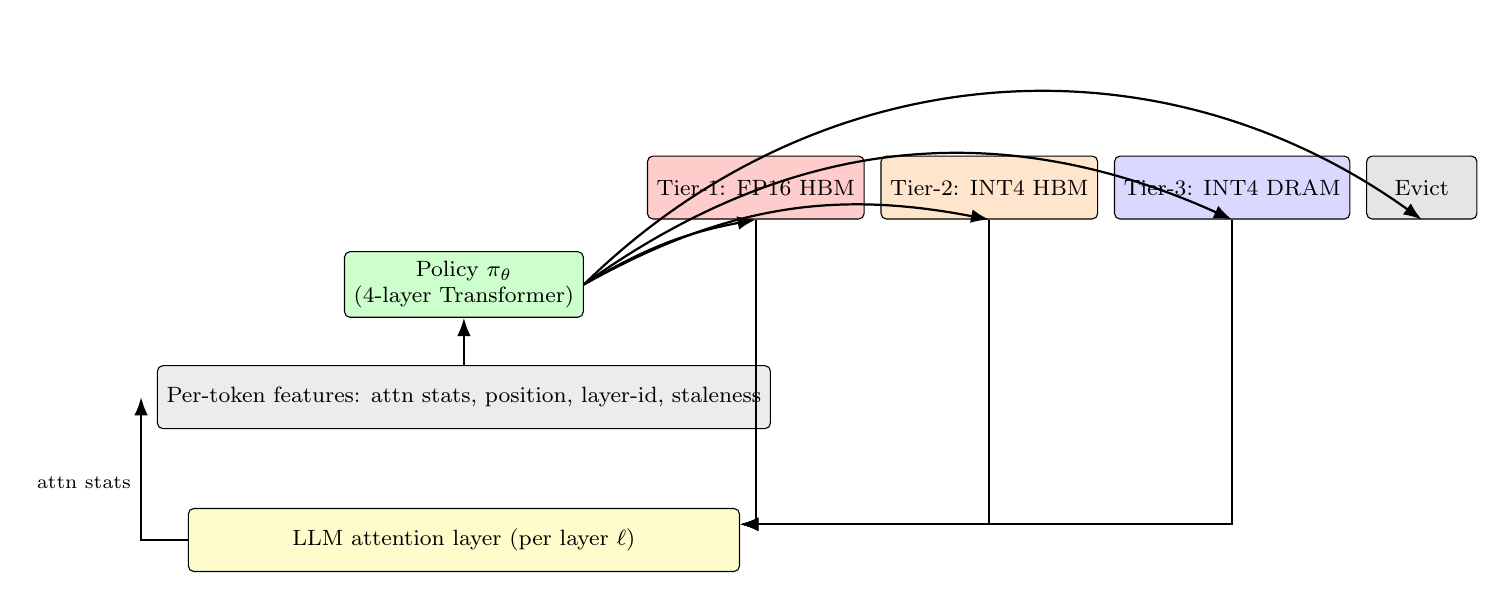
\begin{tikzpicture}[
    >=Latex,
    node distance=4mm and 4mm,
    boxstyle/.style={draw,rounded corners=2pt,minimum height=8mm,align=center,font=\footnotesize},
    tier1/.style={boxstyle,fill=red!20},
    tier2/.style={boxstyle,fill=orange!20},
    tier3/.style={boxstyle,fill=blue!15},
    pol/.style={boxstyle,fill=green!20,minimum width=22mm},
    arr/.style={->,thick}
]
\node[pol] (pol) {Policy $\pi_\theta$\\ (4-layer Transformer)};
\node[boxstyle,below=6mm of pol,fill=gray!15,minimum width=70mm] (feat) {Per-token features: attn stats, position, layer-id, staleness};
\draw[arr] (feat) -- (pol);

\node[tier1,above right=4mm and 8mm of pol,minimum width=22mm] (t1) {Tier-1: FP16 HBM};
\node[tier2,right=2mm of t1,minimum width=22mm] (t2) {Tier-2: INT4 HBM};
\node[tier3,right=2mm of t2,minimum width=22mm] (t3) {Tier-3: INT4 DRAM};
\node[boxstyle,right=2mm of t3,fill=black!10,minimum width=14mm] (ev) {Evict};

\draw[arr,bend left=10] (pol.east) to (t1.south);
\draw[arr,bend left=20] (pol.east) to (t2.south);
\draw[arr,bend left=30] (pol.east) to (t3.south);
\draw[arr,bend left=40] (pol.east) to (ev.south);

\node[boxstyle,below=10mm of feat,fill=yellow!20,minimum width=70mm] (att) {LLM attention layer (per layer $\ell$)};
\draw[arr] (t1.south) |- ([yshift=2mm]att.east) ;
\draw[arr] (t2.south) |- ([yshift=2mm]att.east) ;
\draw[arr] (t3.south) |- ([yshift=2mm]att.east) ;
\draw[arr] (att.west) -| node[left,pos=0.7,font=\scriptsize]{attn stats} ([xshift=-2mm]feat.west);
\end{tikzpicture}
\caption{NeuroKV system architecture. A small Transformer policy network classifies each cached token into one of four hierarchical states based on online attention statistics, position, layer, and staleness. Decisions are reversible: a Tier-3 token can be promoted back to Tier-1 if a future query attends strongly.}
\label{fig:arch}
\end{figure}

\section{Experimental Plan}
\label{sec:exp}

\subsection{Models and Hardware}
Primary: Llama-3-8B-Instruct (32K context) and Mistral-7B-Instruct (32K). Stretch: Llama-3-70B (128K) via tensor parallelism on $2\times$A800. All training and evaluation will run on a single NVIDIA A800 80GB node available through our group's cluster.

\subsection{Benchmarks}
\begin{itemize}
    \item \textbf{LongBench}~\cite{bai2024longbench}: 21 long-context tasks spanning summarization, QA, few-shot learning, and code completion.
    \item \textbf{RULER}~\cite{hsieh2024ruler}: synthetic needle-in-a-haystack at controlled context lengths from 4K to 128K.
    \item \textbf{InfiniteBench}~\cite{zhang2024infinitebench}: tasks beyond 100K tokens.
    \item \textbf{Throughput / latency}: vLLM benchmark suite (sharegpt, longbench-replay) measuring tokens/s, TTFT, ITL, and goodput.
\end{itemize}

\subsection{Baselines}
Full cache (oracle upper bound), random eviction (lower bound), H2O, StreamingLLM, SnapKV, Quest, KIVI (4-bit and 2-bit), and FastGen, all evaluated at matched memory budgets.

\subsection{Metrics}
(i) Task accuracy / ROUGE / F1 / EM at fixed cache budget; (ii) memory--quality Pareto frontier; (iii) end-to-end throughput at fixed quality threshold; (iv) P50/P99 latency; (v) generalization gap (train on LongBench, test on RULER and out-of-distribution code tasks).

\subsection{Ablation Studies}
(a) imitation only vs.\ imitation+RL; (b) policy size (2/4/6 layers, 128/256/512 hidden); (c) per-layer vs.\ shared policy; (d) two-tier vs.\ three-tier hierarchy; (e) feature ablation (remove staleness, remove layer embedding); (f) cross-model transfer (train on Llama-3-8B, deploy on Mistral-7B).

\subsection{Quantitative Targets}
\begin{itemize}
    \item Memory: $4$--$8\times$ effective KV cache reduction vs.\ full cache.
    \item Quality: $\le 1$\,pp average degradation on LongBench at $4\times$ compression.
    \item Throughput: $\ge 1.5\times$ over the strongest published baseline at matched quality.
    \item Generalization: $\le 2$\,pp degradation when transferring policy across model families.
\end{itemize}

\section{Risks and Mitigations}
\begin{itemize}
    \item \textbf{Oracle attribution is expensive.} Mitigation: cache attribution traces; use a 1B-parameter proxy model; subsample to $\le 5{,}000$ training prompts.
    \item \textbf{RL fine-tuning is unstable.} Mitigation: start from imitation policy; clip rewards; use a trust-region (PPO) update; freeze the LLM throughout.
    \item \textbf{Engineering scope (vLLM integration) too large.} Mitigation: implement Stage 1 in plain HuggingFace first; vLLM integration is a stretch goal for week 5--6.
    \item \textbf{Negative result---heuristics are good enough.} Mitigation: even matching the strongest baseline at $\frac{1}{2}$ the memory and producing a clean ablation suite is publishable; the formulation itself is a contribution.
\end{itemize}

\section{Timeline (May 11 -- June 22, 2026)}
\begin{table}[t]
\centering
\caption{Six-week project timeline. The final report (10--16 pages, IEEE Transactions format) is due June 22, 2026.}
\label{tab:gantt}
\renewcommand{\arraystretch}{1.15}
\begin{tabular}{@{}clp{4.6cm}@{}}
\toprule
\textbf{Wk} & \textbf{Dates} & \textbf{Milestone} \\
\midrule
1 & May 11--17 & Literature review; vLLM/HuggingFace environment setup; baseline reproduction harness. \\
2 & May 18--24 & Implement and validate H2O, StreamingLLM, SnapKV, Quest, KIVI baselines. \\
3 & May 25--31 & Oracle attribution pipeline; imitation-learning policy v1 (Stage 1). \\
4 & Jun 1--7   & Three-tier hierarchy; PPO fine-tuning (Stage 2); first end-to-end results. \\
5 & Jun 8--14  & Full evaluation on LongBench / RULER / InfiniteBench; ablations. \\
6 & Jun 15--22 & vLLM integration; throughput measurements; paper writing; code release. \\
\bottomrule
\end{tabular}
\end{table}

\section{Expected Contributions}
\begin{enumerate}
    \item \textbf{Algorithmic:} the first formulation of LLM KV cache management as a constrained sequential decision problem with a three-tier hierarchical action space, solved by a Transformer policy trained with imitation learning followed by quality-aware RL.
    \item \textbf{Systems:} an open-source vLLM extension (\texttt{neurokv-vllm}) that exposes a clean policy interface above the paged-memory layer, enabling future learned policies as drop-in components.
    \item \textbf{Empirical:} a comprehensive Pareto-frontier comparison against six published heuristics on three long-context benchmarks, plus ablations isolating the contribution of each design choice.
    \item \textbf{Reproducibility:} all training scripts, oracle attribution traces, evaluation pipelines, and trained policy checkpoints released under Apache-2.0.
\end{enumerate}

\section{Why this Project Fits the Course}
The project centrally uses deep learning models on two fronts: (a) the policy network is a learned Transformer trained end-to-end with both supervised (imitation) and reinforcement learning objectives, illustrating two paradigms taught in class; and (b) the host LLM is itself a deep Transformer whose internal attention behavior we both probe (for oracle generation) and control (via the policy). The work is firmly in AI infrastructure---a current research frontier with direct industrial relevance---and it aligns with the grading criteria of (i) novelty, (ii) creativity in problem formulation, (iii) systematic experimental analysis, (iv) code reproducibility, and (v) report readability.

\bibliographystyle{IEEEtran}
\bibliography{references}

\end{document}
